Прогресс в области машинного обучения и разработки интеллектуальных ассистентов ведет к росту потребности в
высококачественных корпусах текстов и аннотированных изображений. Обучение на предметном корпусе
позволяет улучшать количественные метрические показатели достоверности передаваемых знаний 
на десятки процентных пунктов \cite{tinn2023fine}. Тем не менее открытые корпусы русского языка 
\cite{hung2022multi2woz} \cite{dmitrieva2023automatic} \cite{ivanov2023new} почти не содержат образовательной тематики.
Представленный в секции корпус является вариантом решения проблемы недостатка данных в направлении образования. 
Результаты моделирования предоставлены на открытых ресурсах\footnote{
\url{https://github.com/NMashalov/Generative-modeling-appliance-for-creating-educational-tasks}
и \url{https://huggingface.co/datasets/NMashalov/task_illustrations_dataset}
} с указанием источников данных \ref{literature}. Полученный корпус имеет мощность порядка миллиона слов и десятка тысяч изображений. На рисунке \ref{distribution} приведено
распределение по источникам данных, включающее открытые цифровые документы, адаптированные с других языков корпусы и естественно-научные 
журналы.
\begin{figure}[h]
    \centering
    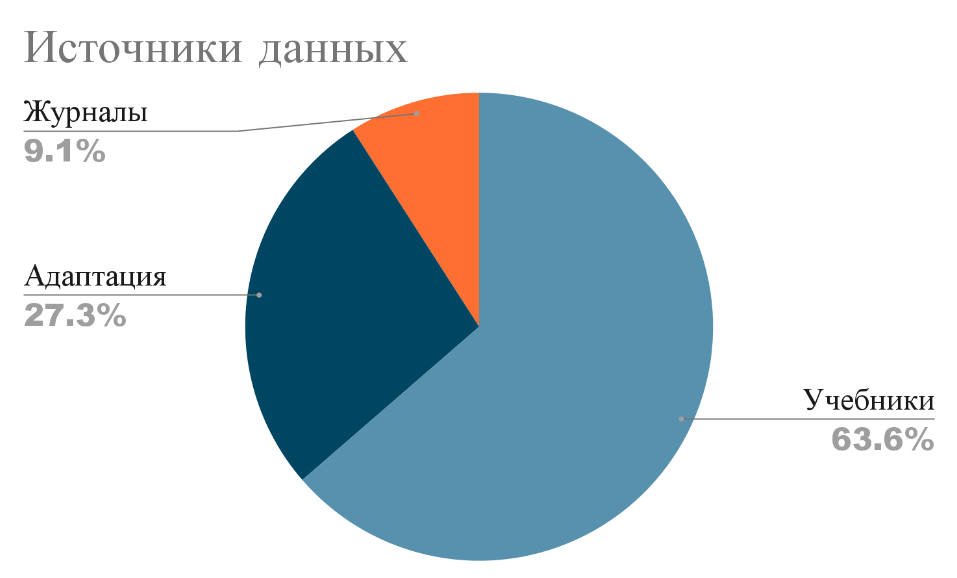
\includegraphics[width=0.5\textwidth]{assets/work/dataset/diagram.png}
    \caption{Распределение данных по источникам.}
    \label{distribution}
\end{figure}